% https://tikz.net/electromagnetic_spectrum/
% Author: Izaak Neutelings (May 2020)
\documentclass[tikz]{standalone}
\tikzset{>=latex} % for LaTeX arrow head
\usepackage{ifthen}
\usepackage{xcolor}
\usepackage{physics}
\usepackage{siunitx}

\colorlet{wavecol}{orange!35!black}
\colorlet{freqcol}{green!25!black}
\colorlet{enercol}{blue!35!black}
\pgfdeclareverticalshading{rainbow}{100bp}{
  color(0bp)=(red); color(25bp)=(red); color(35bp)=(yellow);
  color(45bp)=(green); color(55bp)=(cyan); color(65bp)=(blue);
  color(75bp)=(violet); color(100bp)=(violet)
}


\begin{document}


% ELECTROMAGNETIC SPECTRUM
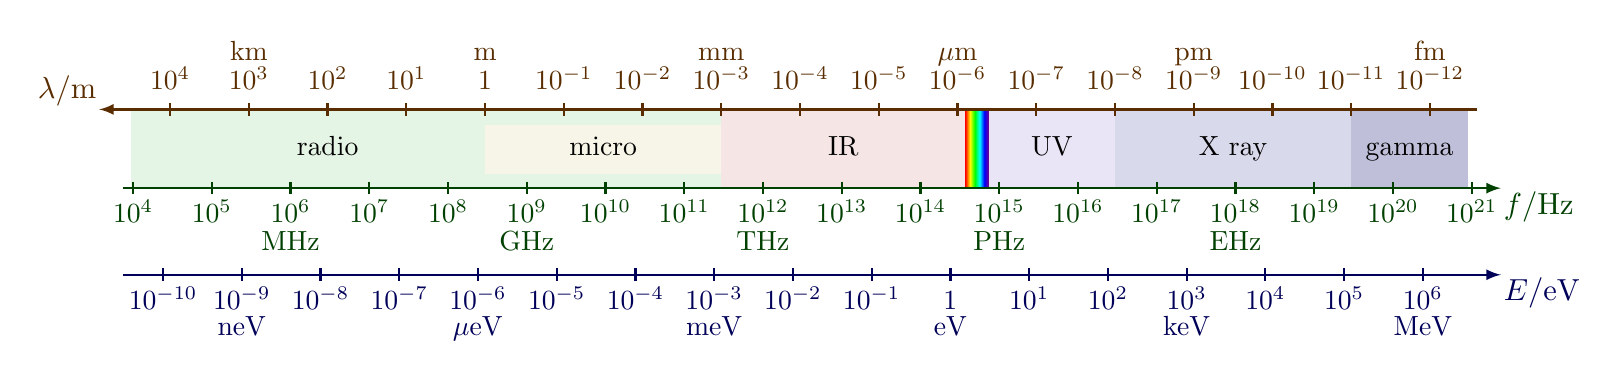
\begin{tikzpicture}[xscale=1]
  \def\h{1}
  \def\radio{-4}
  \def\micro{0}
  \def\IR{3}
  \def\red{6.10}  % log(700e-9) = -6.15490196
  \def\blue{6.40} % log(400e-9) = -6.39794001
  \def\UV{6.40}
  \def\Xray{8}
  \def\gamm{11}
  \def\last{12}
  \def\radiof{-5}
  \def\dx{0.6}
  \def\yE{-1.1*\h}
  
  \def\tick#1#2#3{\draw[thick,#2] (#1+.08) --++ (0,-.16) node[below=-2pt,scale=1] {\strut #3};}
  \def\ticka#1#2#3{\draw[thick,#2] (#1+.08) --++ (0,-.16) node[above=2pt,scale=1] {\strut #3};}
  
  % MIDDLE
  \fill[green!60!black!10] (\radio-0.82*\dx,0) rectangle (\IR,\h);
  \fill[yellow!60!black!10] (\micro,0.18*\h) rectangle (\IR,0.8*\h);
  \fill[red!60!black!10] (\IR,0) rectangle (\red,\h);
  \fill[blue!60!violet!80!black!10] (\UV,0) rectangle (\Xray,\h);
  \fill[blue!50!black!15] (\Xray,0) rectangle (\gamm,\h);
  \fill[blue!40!black!25] (\gamm,0) rectangle (\last+0.8*\dx,\h);
  \shade[shading=rainbow,shading angle=-90] (\red,0) rectangle (\blue,\h);
  \node at ({(\radio+\micro)/2},\h/2) {\strut radio};
  \node at ({(\micro+\IR)/2},   \h/2) {\strut micro};
  \node at ({(\IR+\red)/2},     \h/2) {\strut IR};
  %\node at (\red,  \h/2) {red};
  %\node at (\red,  \h/2) {blue};
  \node at ({(\UV+\Xray)/2},    \h/2) {\strut UV};
  \node at ({(\Xray+\gamm)/2},  \h/2) {\strut X ray};
  \node at ({(\gamm+\last+0.8*\dx)/2},  \h/2) {\strut gamma};
  
  % WAVELENGTH
  \draw[->,thick,wavecol] (\last+\dx,\h) -- (\radio-1.5*\dx,\h) node[above left=-3,scale=1.1] {$\lambda$/\si{m}};
  \foreach \x [evaluate={\i=int(-\x)}] in {\radio,...,\last}{
    \ifthenelse{\i=0}{ \ticka{\x,\h}{wavecol}{$1$} }
                     { \ticka{\x,\h}{wavecol}{$10^{\i}$} }
  }
  \node[wavecol,scale=1] at (-3,1.71*\h) {\strut km};
  \node[wavecol,scale=1] at ( 0,1.71*\h) {\strut m};
  \node[wavecol,scale=1] at ( 3,1.71*\h) {\strut mm};
  \node[wavecol,scale=1] at ( 6,1.71*\h) {\strut \si{\mu m}};
  \node[wavecol,scale=1] at ( 9,1.71*\h) {\strut pm};
  \node[wavecol,scale=1] at (12,1.71*\h) {\strut fm};
  %\node[wavecol,scale=1] at (15,1.71*\h) {\strut am};
  
  % FREQUENCY
  % log(f) = log(c) - log(lambda)
  % log(c) = log(2.997e8) = 8.4766867429
  \draw[->,thick,freqcol] (\radio-\dx,0) -- (\last+1.5*\dx,0) node[below right=-3,scale=1.1] {$f$/\si{Hz}};
  \foreach \x [evaluate={\i=int(\x+9);\X=\x+0.53}] in {\radiof,...,\last}{
    \tick{\X,0}{freqcol}{$10^{\i}$}
  }
  %\node[freqcol,scale=1] at (-8.47+ 3,-0.65*\h) {\strut kHz};
  \node[freqcol,scale=1] at (-8.47+ 6,-0.71*\h) {\strut MHz};
  \node[freqcol,scale=1] at (-8.47+ 9,-0.71*\h) {\strut GHz};
  \node[freqcol,scale=1] at (-8.47+12,-0.71*\h) {\strut THz};
  \node[freqcol,scale=1] at (-8.47+15,-0.71*\h) {\strut PHz};
  \node[freqcol,scale=1] at (-8.47+18,-0.71*\h) {\strut EHz};
  
  % ENERGY
  % log(E) = log(hc) - log(lambda)
  % log(hc) = log(2.997e8*4.135e-15) = -5.9068377432
  \draw[->,thick,enercol] (\radio-\dx,\yE) -- (\last+1.5*\dx,\yE) node[below right=-3,scale=1.1] {$E$/\si{eV}};
  \foreach \x [evaluate={\i=int(\x-6);\X=\x-0.09}] in {\radio,...,\last}{
    \ifthenelse{\i=0}{ \tick{\X,\yE}{enercol}{$1$} }
                     { \tick{\X,\yE}{enercol}{$10^{\i}$} }
  }
  %\node[enercol,scale=1] at (5.91-15,\yE-0.69*\h) {\strut feV};
  %\node[enercol,scale=1] at (5.91-12,\yE-0.69*\h) {\strut peV};
  \node[enercol,scale=1] at (5.91- 9,\yE-0.69*\h) {\strut neV};
  \node[enercol,scale=1] at (5.91- 6,\yE-0.69*\h) {\strut \si{\mu eV}};
  \node[enercol,scale=1] at (5.91- 3,\yE-0.69*\h) {\strut meV};
  \node[enercol,scale=1] at (5.91+ 0,\yE-0.69*\h) {\strut  eV};
  \node[enercol,scale=1] at (5.91+ 3,\yE-0.69*\h) {\strut keV};
  \node[enercol,scale=1] at (5.91+ 6,\yE-0.69*\h) {\strut MeV};
  %\node[enercol,scale=1] at (5.91+9,\yE-0.69*\h) {\strut GeV};
  
\end{tikzpicture}


\end{document}